% ========== 基础功能示例 ==========
\documentclass[../main]{subfiles}
\begin{document}

\section{基础排版与文本结构}

\subsection{段落与文本格式}
这是段落示例,LaTeX自动处理段落间距和断行。可以使用\highlight{高亮文本}来强调重要内容。

\notebox{这是一个注意事项框,可以用来提醒读者重要信息。}

\subsection{增强列表环境}
无序列表示例:
\begin{itemize}
    \item 条目一 - 包含更好的间距
    \item 条目二 - 自动优化排版
        \begin{itemize}
            \item 子条目A
            \item 子条目B
        \end{itemize}
    \item 条目三 - 支持更多自定义
\end{itemize}

编号列表(带自定义格式):
\begin{enumerate}[label=(\arabic*)]
    \item 第一点
    \item 第二点
    \item 第三点
\end{enumerate}

传统编号列表:
\begin{enumerate}
    \item 第一点
    \item 第二点
    \item 第三点
\end{enumerate}

\section{数学与定理环境}

\subsection{基础数学公式}
行内公式:$E=mc^2$,行间公式如下:
\begin{equation}\label{eq:gravity}
    F = G\frac{m_1 m_2}{r^2}
\end{equation}

多行公式:
\begin{align}
    \nabla \times \vec{E} &= -\frac{\partial \vec{B}}{\partial t} \label{eq:faraday}\\
    \nabla \times \vec{B} &= \mu_0\vec{J} + \mu_0\epsilon_0\frac{\partial \vec{E}}{\partial t} \label{eq:ampere}
\end{align}

引用公式:参见公式\cref{eq:gravity}。

\subsection{定理环境示例}

\begin{definition}[拉格朗日中值定理]
若函数 $f(x)$ 在闭区间 $[a,b]$ 上连续,在开区间 $(a,b)$ 内可导,则存在 $\xi \in (a,b)$,使得:
$$f'(\xi) = \frac{f(b) - f(a)}{b - a}$$
\end{definition}

\begin{theorem}[费马小定理]
若 $p$ 是素数,$a$ 是不被 $p$ 整除的整数,则:
$$a^{p-1} \equiv 1 \pmod{p}$$
\end{theorem}

\begin{example}
计算 $3^{10} \bmod 11$:
由于 $11$ 是素数且 $\gcd(3,11)=1$,根据费马小定理:
$$3^{10} \equiv 1 \pmod{11}$$
\end{example}

% ========== 算法与可视化 ==========
\section{算法与流程图}

\subsection{算法伪代码}

\begin{algorithm}[H]
\caption{快速排序算法}
\label{alg:quicksort}
\KwIn{数组 $A[1..n]$,起始索引 $p$,结束索引 $r$}
\KwOut{排序后的数组}

\Fn{\FMain{$A, p, r$}}{
    \If{$p < r$}{
        $q \leftarrow$ PARTITION$(A, p, r)$\;
        QUICKSORT$(A, p, q-1)$\;
        QUICKSORT$(A, q+1, r)$\;
    }
}

\Fn{PARTITION$(A, p, r)$}{
    $x \leftarrow A[r]$\;
    $i \leftarrow p - 1$\;
    \For{$j \leftarrow p$ \KwTo $r-1$}{
        \If{$A[j] \leq x$}{
            $i \leftarrow i + 1$\;
            交换 $A[i]$ 和 $A[j]$\;
        }
    }
    交换 $A[i+1]$ 和 $A[r]$\;
    \Return $i + 1$\;
}
\end{algorithm}

\subsection{流程图示例}

\begin{figure}[H]
\centering
\begin{tikzpicture}[node distance=2cm]
    \tikzstyle{startstop} = [rectangle, rounded corners, minimum width=3cm, minimum height=1cm, text centered, draw=black, fill=red!30]
    \tikzstyle{process} = [rectangle, minimum width=3cm, minimum height=1cm, text centered, draw=black, fill=orange!30]
    \tikzstyle{decision} = [diamond, minimum width=3cm, minimum height=1cm, text centered, draw=black, fill=green!30]
    \tikzstyle{arrow} = [thick,->,>=stealth]

    \node (start) [startstop] {开始};
    \node (input) [process, below of=start] {输入数据};
    \node (decide) [decision, below of=input, yshift=-0.5cm] {条件判断};
    \node (process1) [process, below of=decide, yshift=-0.5cm] {处理A};
    \node (process2) [process, right of=decide, xshift=2cm] {处理B};
    \node (stop) [startstop, below of=process1] {结束};

    \draw [arrow] (start) -- (input);
    \draw [arrow] (input) -- (decide);
    \draw [arrow] (decide) -- node[anchor=east] {是} (process1);
    \draw [arrow] (decide) -- node[anchor=south] {否} (process2);
    \draw [arrow] (process1) -- (stop);
    \draw [arrow] (process2) |- (stop);
\end{tikzpicture}
\caption{算法流程图示例}
\label{fig:flowchart}
\end{figure}

\section{数据可视化}

\subsection{函数图像}

\begin{figure}[H]
\centering
\begin{tikzpicture}
\begin{axis}[
    title={三角函数图像},
    xlabel={$x$},
    ylabel={$y$},
    xmin=-2*pi, xmax=2*pi,
    ymin=-1.5, ymax=1.5,
    xtick={-6.28318, -3.14159, 0, 3.14159, 6.28318},
    xticklabels={$-2\pi$, $-\pi$, $0$, $\pi$, $2\pi$},
    grid=major,
    legend pos=north west
]
    \addplot[color=red, domain=-2*pi:2*pi, samples=100] {sin(deg(x))};
    \addplot[color=blue, domain=-2*pi:2*pi, samples=100] {cos(deg(x))};
    \legend{$\sin(x)$, $\cos(x)$}
\end{axis}
\end{tikzpicture}
\caption{正弦和余弦函数图像}
\label{fig:trigfunctions}
\end{figure}

\subsection{数据图表}

\begin{figure}[H]
\centering
\begin{tikzpicture}
\begin{axis}[
    title={实验数据分析},
    xlabel={时间 (s)},
    ylabel={温度 ($^\circ$C)},
    grid=major,
    legend pos=north east
]
    \addplot[color=red, mark=square] coordinates {
        (0,20) (1,25) (2,32) (3,38) (4,42) (5,45) (6,47) (7,48) (8,49) (9,50)
    };
    \addplot[color=blue, mark=circle] coordinates {
        (0,18) (1,22) (2,28) (3,35) (4,40) (5,43) (6,45) (7,46) (8,47) (9,48)
    };
    \legend{实验组, 对照组}
\end{axis}
\end{tikzpicture}
\caption{温度变化对比实验}
\label{fig:temperature}
\end{figure}

% ========== 图表与代码 ==========
\section{图形插入与管理}

本模板提供了多种插入和管理图形的方式,以满足不同场景的需求。

\subsection{基础图片插入}
最基础的图片插入方式是使用 \texttt{figure} 环境和 \texttt{\textbackslash includegraphics} 命令。这提供了最大的灵活性。
\begin{figure}[H]
    \centering % 图片居中
    
\includegraphics[width=0.5\textwidth]{figure/badge-horizonal.pdf}
    \caption{基础图片插入示例}
    \label{fig:basic-image}
\end{figure}

可以交叉引用此图片,例如:图\cref{fig:basic-image}。

\subsection{使用自定义命令 \texttt{\textbackslash insertfig}}
为了简化操作,模板定义了 \texttt{\textbackslash insertfig} 命令,可以快速插入带标题和标签的居中图片。

\insertfig{figure/badge.pdf}{使用 insertfig 命令插入的图片}{fig:insertfig-command}

这条命令等效于:
\begin{verbatim}
\begin{figure}[H]
    \centering
    
\includegraphics[width=0.8\textwidth]{figure/badge.pdf}
    \caption{使用 insertfig 命令插入的图片}
    \label{fig:insertfig-command}
\end{figure}
\end{verbatim}
你也可以指定图片宽度,例如 \texttt{\textbackslash insertfig[0.6]\{...\}} 将设置宽度为页面宽度的60\%。

\subsection{图片参数调整}
\texttt{\textbackslash includegraphics} 命令支持多种参数来调整图片样式:
\begin{itemize}
    \item \texttt{width}: 按宽度缩放,例如 \texttt{width=0.3\textbackslash textwidth}。
    \item \texttt{height}: 按高度缩放,例如 \texttt{height=4cm}。
    \item \texttt{scale}: 按比例缩放,例如 \texttt{scale=0.5}。
    \item \texttt{angle}: 旋转图片,例如 \texttt{angle=45}。
\end{itemize}

\begin{figure}[H]
    \centering
    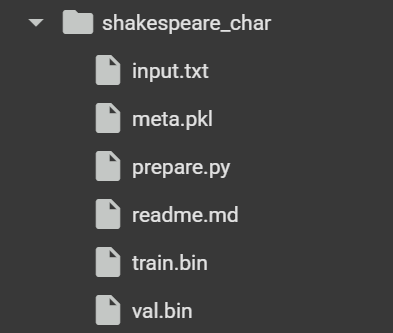
\includegraphics[width=0.4\textwidth, angle=15]{figure/template/2025-05-19 232610.png}
    \caption{调整宽度并旋转15度的图片}
    \label{fig:rotated-image}
\end{figure}

\subsection{并排插入多个图片}
使用 \texttt{subcaption} 宏包提供的 \texttt{subfigure} 环境,可以方便地将多个图片并排显示,并为它们分别添加子标题。

\begin{figure}[H]
    \centering
    \begin{subfigure}{0.45\textwidth}
        \centering
        
\includegraphics[width=\linewidth]{figure/badge.pdf}
        \caption{第一个子图}
        \label{fig:subfig-a}
    \end{subfigure}
    \hfill % 在子图之间添加一些水平间距
    \begin{subfigure}{0.45\textwidth}
        \centering
        
\includegraphics[width=\linewidth]{figure/badge-horizonal.pdf}
        \caption{第二个子图}
        \label{fig:subfig-b}
    \end{subfigure}
    \caption{并排显示的两个图片}
    \label{fig:side-by-side}
\end{figure}

可以单独引用子图,如 \cref{fig:subfig-a},也可以引用整个图组,如 \cref{fig:side-by-side}。

\subsection{图片浮动位置控制}
LaTeX 提供了多种浮动位置参数来控制图片的放置位置:
\begin{itemize}
    \item \texttt{[H]}: 强制在当前位置(需要 float 宏包)
    \item \texttt{[htbp]}: 依次尝试当前位置、页面顶部、页面底部、单独页面
    \item \texttt{[!h]}: 忽略一些浮动规则,强制在当前位置
\end{itemize}

\begin{figure}[htbp]
    \centering
    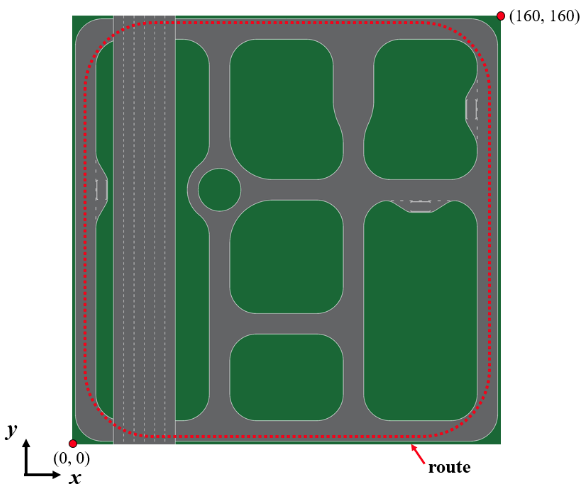
\includegraphics[width=0.3\textwidth]{figure/template/2025-05-27 082408.png}
    \caption{使用 htbp 浮动位置参数的图片}
    \label{fig:float-example}
\end{figure}

\subsection{多图网格布局}
当需要展示多个相关图片时,可以使用网格布局:

\begin{figure}[H]
    \centering
    \begin{subfigure}{0.3\textwidth}
        \centering
        
\includegraphics[width=\linewidth]{figure/badge.pdf}
        \caption{图A}
        \label{fig:grid-a}
    \end{subfigure}
    \hfill
    \begin{subfigure}{0.3\textwidth}
        \centering
        
\includegraphics[width=\linewidth]{figure/badge-horizonal.pdf}
        \caption{图B}
        \label{fig:grid-b}
    \end{subfigure}
    \hfill
    \begin{subfigure}{0.3\textwidth}
        \centering
        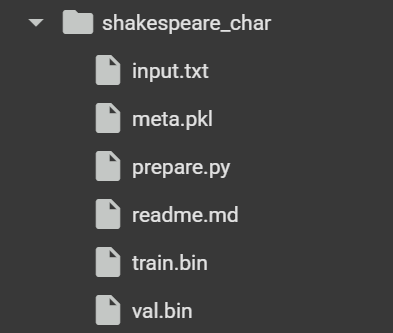
\includegraphics[width=\linewidth]{figure/template/2025-05-19 232610.png}
        \caption{图C}
        \label{fig:grid-c}
    \end{subfigure}
    
    \vspace{0.5cm} % 添加垂直间距
    
    \begin{subfigure}{0.45\textwidth}
        \centering
        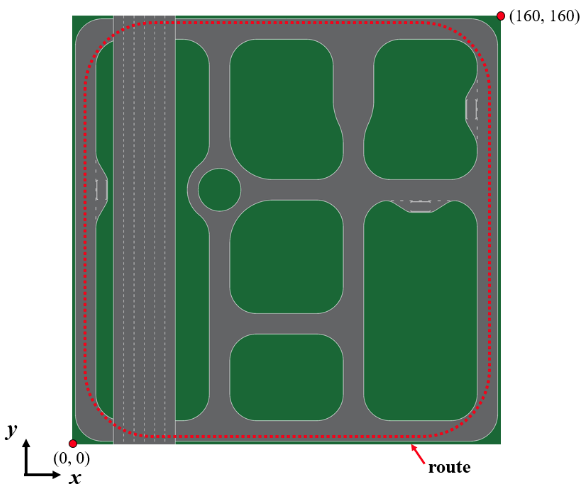
\includegraphics[width=\linewidth]{figure/template/2025-05-27 082408.png}
        \caption{图D}
        \label{fig:grid-d}
    \end{subfigure}
    \hfill
    \begin{subfigure}{0.45\textwidth}
        \centering
        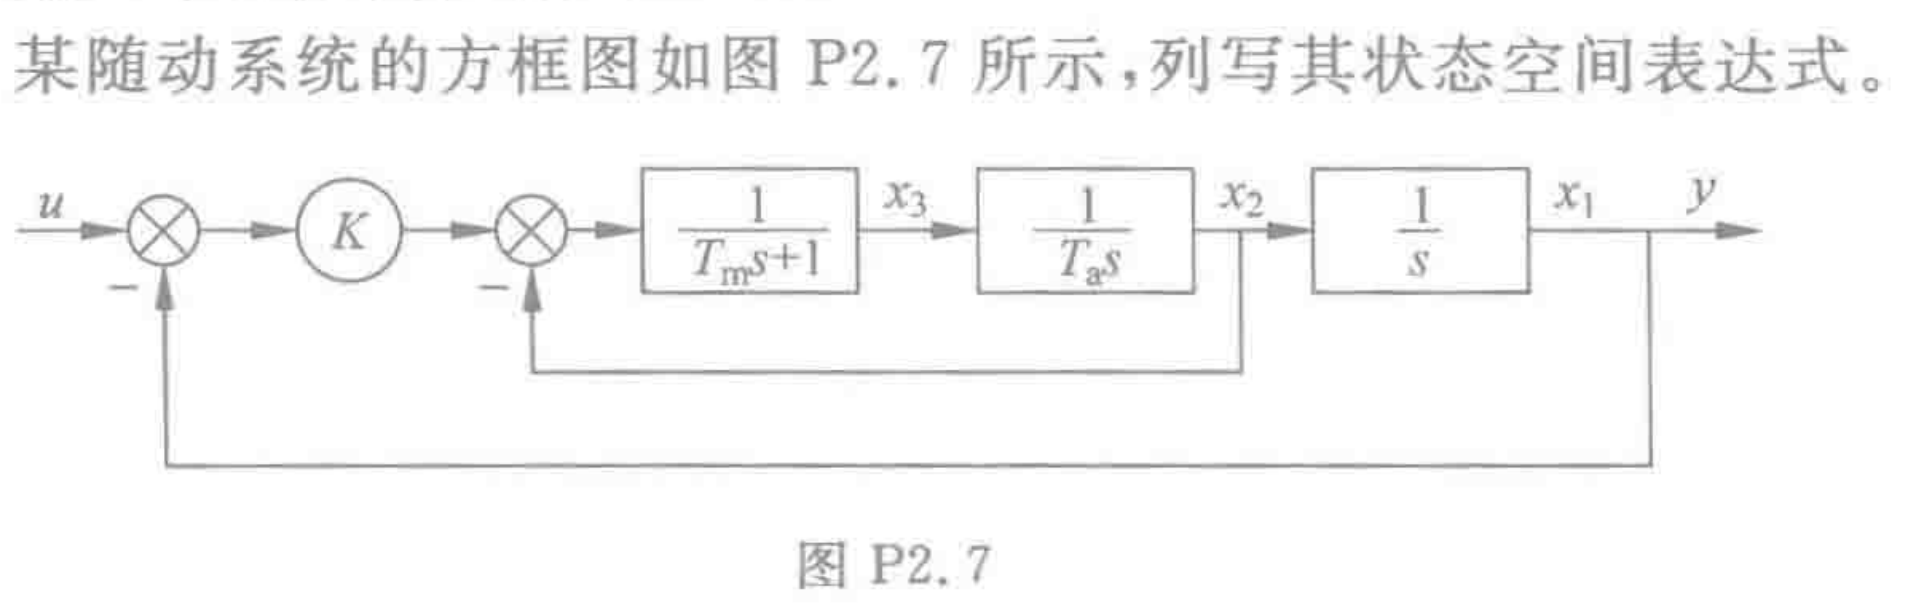
\includegraphics[width=\linewidth]{figure/template/20250402171850.png}
        \caption{图E}
        \label{fig:grid-e}
    \end{subfigure}
    
    \caption{多图网格布局示例}
    \label{fig:grid-layout}
\end{figure}

\subsection{图片路径管理}
本模板的图片建议按以下结构组织:
\begin{itemize}
    \item \texttt{figure/} - 主要图片目录
    \item \texttt{figure/ch1/}, \texttt{figure/ch2/} - 按章节分类
    \item \texttt{figure/template/} - 模板示例图片
\end{itemize}

引用时可以使用相对路径:
\begin{lstlisting}[language=TeX, basicstyle=\ttfamily\small]
\includegraphics{figure/ch1/diagram.png}
\includegraphics{figure/template/example.png}
\end{lstlisting}

\subsection{图片引用与标注}
使用 \texttt{cleveref} 宏包可以实现智能引用:
\begin{itemize}
    \item 单个引用:\cref{fig:basic-image}
    \item 多个引用:\cref{fig:grid-a,fig:grid-b,fig:grid-c}
    \item 范围引用:\cref{fig:subfig-a,fig:subfig-b}
\end{itemize}

引用整个图组:参见\cref{fig:grid-layout}展示了多种图片的网格布局效果。

\section{表格设计与制作}

\subsection{三线表}
标准三线表示例:
\begin{table}[H]
    \centering
    \caption{三线表示例}
    \label{tab:booktabs}
    \begin{tabular}{lccr}
        \toprule
        姓名 & 年龄 & 专业 & 绩点 \\
        \midrule
        张三 & 20 & 计算机科学 & 3.85 \\
        李四 & 21 & 物理学 & 3.92 \\
        王五 & 19 & 数学 & 3.78 \\
        \bottomrule
    \end{tabular}
\end{table}

\subsection{自适应表格}
自适应宽度表格示例:
\begin{table}[H]
    \centering
    \caption{自适应宽度表格}
    \label{tab:tabularx}
    \begin{tabularx}{\tablewidth}{|l|X|X|}
        \hline
        \textbf{优先级} & \textbf{任务描述} & \textbf{备注} \\
        \hline
        高 & 完成项目核心功能开发 & 预计耗时3天 \\
        \hline
        中 & 撰写项目文档 & 无 \\
        \hline
        低 & 优化用户界面 & 可选 \\
        \hline
    \end{tabularx}
\end{table}

\subsection{长表格示例}

% 双栏布局下将长表格改为普通表格以避免兼容性问题
\begin{table}[H]
    \centering
    \caption{学生成绩统计表(双栏兼容版本)}
    \label{tab:grades-twocolumn}
    \begin{tabularx}{\linewidth}{|l|X|X|r|}
        \hline
        \textbf{姓名} & \textbf{数学} & \textbf{物理} & \textbf{总分} \\
        \hline
        张三 & 95 & 88 & 183 \\
        李四 & 87 & 92 & 179 \\
        王五 & 91 & 85 & 176 \\
        赵六 & 89 & 90 & 179 \\
        钱七 & 93 & 87 & 180 \\
        \hline
    \end{tabularx}
\end{table}

\subsection{算法复杂度分析}

\begin{table}[H]
\centering
\caption{常见排序算法复杂度对比}
\label{tab:algorithm-complexity}
\begin{tabular}{@{}lcccc@{}}
\toprule
\textbf{算法} & \textbf{最佳情况} & \textbf{平均情况} & \textbf{最坏情况} & \textbf{空间复杂度} \\
\midrule
冒泡排序 & $O(n)$ & $O(n^2)$ & $O(n^2)$ & $O(1)$ \\
选择排序 & $O(n^2)$ & $O(n^2)$ & $O(n^2)$ & $O(1)$ \\
插入排序 & $O(n)$ & $O(n^2)$ & $O(n^2)$ & $O(1)$ \\
快速排序 & $O(n\log n)$ & $O(n\log n)$ & $O(n^2)$ & $O(\log n)$ \\
归并排序 & $O(n\log n)$ & $O(n\log n)$ & $O(n\log n)$ & $O(n)$ \\
堆排序 & $O(n\log n)$ & $O(n\log n)$ & $O(n\log n)$ & $O(1)$ \\
\bottomrule
\end{tabular}
\end{table}

\section{代码块与行内代码}

\subsection{代码块对比示例}

\paragraph{Listings 代码块}
适合需要更多自定义选项的场景:
\begin{lstlisting}[language=Python, caption=Python 函数示例]
def process_data(input_data, configuration_parameters,
                output_format="json", verbose=True):
    """处理数据的函数示例"""
    if verbose:
        print(f"处理 {len(input_data)} 条数据记录")
    return processed_result
\end{lstlisting}

JavaScript 示例:
\begin{lstlisting}[language=JavaScript, caption=JavaScript 链式调用示例]
const result = someObject
    .method(param1, param2, param3)
    .anotherMethod(moreParams);
\end{lstlisting}

\subsection{行内代码}

Listings 行内代码示例:\lstinline{y = [i**3 for i in range(5)]}

\subsubsection{长代码行内显示解决方案}

\paragraph{解决方案1:使用缩写或省略}
对于超长函数名,可以使用缩写或在代码后加注释说明。

\paragraph{解决方案2:使用 lstinline 替代}
使用 \texttt{listings} 包的行内代码,支持自动换行:\\
\lstinline[breaklines=true]{calculate_complex_exprrrrrrrrrrrrrrrrrrrrrrrrrrrrrrrrrrrrr(x=10, y=20, z=30, alpha=0.5, beta=0.7)}

\subsubsection{长代码处理}
超长代码的另一种处理方法 (listings 方案):
\begin{lstlisting}[language=Python, caption=长变量名示例 (listings), basicstyle=\ttfamily\footnotesize\CJKfamily{zhkai}, breaklines=true, breakatwhitespace=false, showstringspaces=false, literate={_}{{\_}}1]
very_long_variable_name_example = "这是一个非常长长长长长长长长长长长长长长长长长长长长长长长长长长长长长长长长长长长长长长长长长长长长长长长长长长长长长长长长长长长长长长长长长长的变量名示例"
\end{lstlisting}

% ========== 高级功能 ==========
\section{高级功能与文档收尾}

\subsection{超链接与交互}
网址链接:\url{https://www.sysu.edu.cn/}

自定义链接:\href{https://www.sysu.edu.cn/}{中山大学官网}

\subsection{排版与使用例}
超长无空格文本换行示例:\seqsplit{PPPPPPPPPPPPPPPPPneumonoultramicroscopicsilicovolcanoconiosisExample}

物理量示例:光速约为\SI{3.00e8}{\meter\per\second},温度\SI{100}{\degreeCelsius}。

光速:\SI{2.998e8}{\meter\per\second}

温度:\SI{100}{\degreeCelsius} = \SI{373.15}{\kelvin}

电阻:\SI{1.5}{\kilo\ohm}

\subsection{参考文献管理}
单个引用:\autocite{knuth1986texbook}

多个引用:\autocite{vaswani2017attention,brown2020language}

带页码引用:\autocite[第35页]{wang2010zhongwen}

文本式引用:\textcite{knuth1986texbook}详细介绍了TeX系统。

\subsection{交叉引用示例}
智能交叉引用:参见\cref{fig:basic-image,tab:booktabs,eq:gravity}。

参考算法:\cref{alg:quicksort}展示了快速排序的实现。

参考图表:\cref{fig:temperature,tab:algorithm-complexity}显示了实验数据和算法对比。

参考公式:根据\cref{eq:gravity,eq:faraday}可以看出物理定律的数学表达。

\end{document} 